\chapter{Steady-state dynamics of the audience applause}
\label{chap3}

\hspace{\parindent} A system is in steady-state when its behavior no longer changes in time. In the context of a real audience applause, the system rapidly spikes up in the number of people applauding, fluctuates, then slowly dies down till everyone stops clapping. This setup has the trivial steady-state of $0$.
However, simulations have shown that there are parameters where the steady-state is not zero, corresponding to $n_{c}$ people clapping indefinitely.
The value can be calculated by equating either \eqref{eq:diff1} or \eqref{eq:diff2} to zero, plugging in the given parameters $a, b, \alpha, \beta$, and then solving for $n_{c}$.

\section{Steady-state equation for different cases}

\hspace{\parindent} The steady-state conditions are when the state $\vec{n}$ is fixed and when the forcing function expires. 
This is when $d\vec{n}/dt = 0$ and when $f=0$.
The derivation is shown in the appendix (\ref{apndx:derivSS})
Once these conditions are achieved, \eqref{eq:diff1} and \eqref{eq:diff2} are simplified to the steady-state equation for $n_c$:

\begin{equation}\label{eq:steadystate}
\bar{a}(N-n_{c})(N-1 + \beta n_{c}) = b(N-1)^{2}
\end{equation}

where $\bar{a}\equiv a\alpha$. 
The values of steady state $n_{c}$ may be solved for any given $\bar{a},b,$ and $\beta$.
Parametrizing \eqref{eq:steadystate} to time gives the phases space plot for the given parameters $b$ and $\beta$, shown in figure \ref{fig:phaseSpace}.
The phase space plots for various $b$ values are shown in Appendix \ref{apndx:phasespace}
Though the trivial steady-state solution is not included in \eqref{eq:steadystate}, it has been included in the phase space.
The coordinate ($\bar{a}$,$n_{c}$) on the curves represent the $n_{c}$ value for a given $\bar{a}$ value at the given $b$ and $\beta$ value, where $\beta$ is the color of the curve.
Values below $0$ are extraneous since $n_{c}$ refers to the number of people clapping, which cannot be negative.
This means that there are two possible steady-state values for $\beta \leq 1$, the trivial solution $0$, and the non-trivial solution found on the appropriate curve.
On the other hand, there are three possible steady-state values for $\beta > 1$, the trivial solution $0$, and two non-trivial solutions found on the appropriate curve.

\begin{figure}
 \centering
  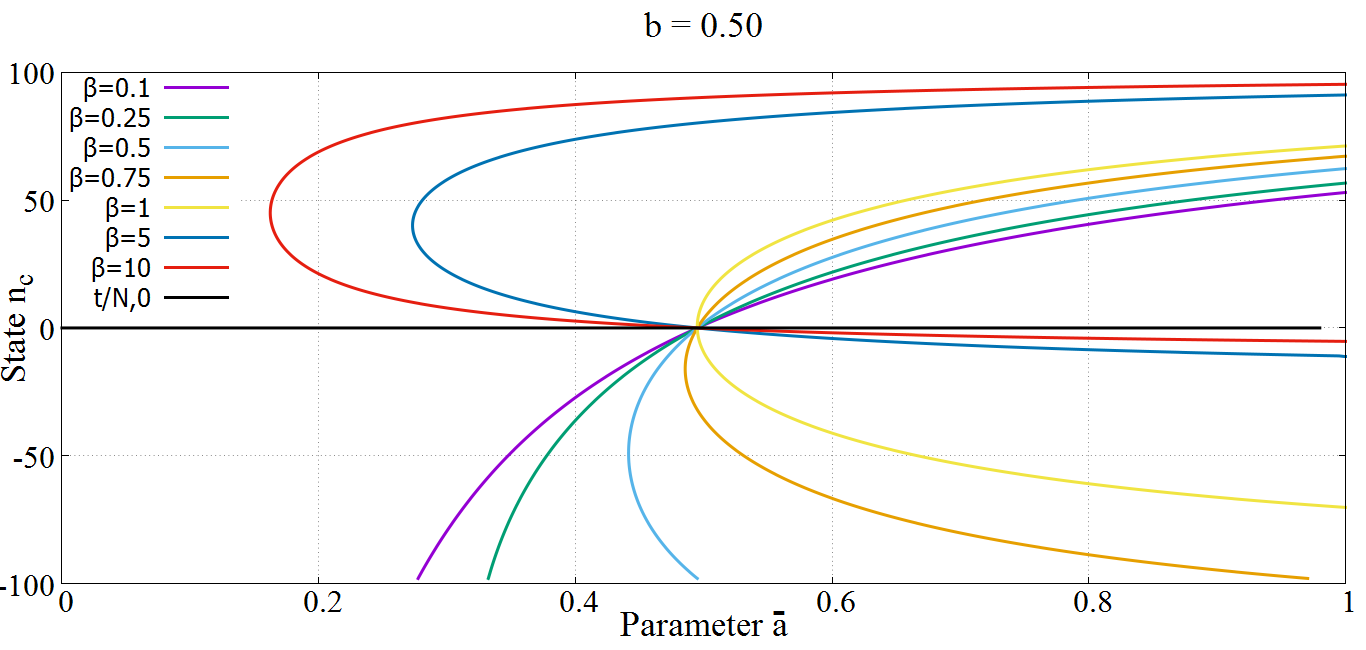
\includegraphics[width=\linewidth]{images/chapter3/phaseSpace.png}
  \caption{The phase space plot of the steady-state value $n_{c}$ versus $\bar{a}$ for various $\beta$ values and $b = 0.5$. Included is the trivial steaty-state solution $n_{c} = 0$}
  \label{fig:phaseSpace}
\end{figure}

\subsection{Bifurcation Theory}
\hspace{\parindent}Given a specific parameter set $(a,b,\alpha,\beta)$, the steady-state solution can only either be the trivial ($0$, in black) or non-trivial, never both. How this is determined falls under bifurcation theory. 
This refers to the study of change to the state of the system as a parameter or parameters are changed and can be applied to steady-state systems \cite{bifurcation}.
The system is analyzed to find out where the change occurs and if there are stability changes.


\subsection{Critical Points}
\hspace{\parindent}From observing all phase space plots of various $b$ values, all $\beta$ curves intersect, along with the trivial solution, at a specific point.
Setting $n_{c} = 0$ in \eqref{eq:steadystate} gives us this critical point of intersection, $\bar{a}_{1}$:

\begin{equation}
\bar{a}_{1} = \frac{b(N-1)}{N}
\end{equation}

which for $N\gg1$ results to the observed $\bar{a}_{1}\approx b$. Solution for the critical point is shown in Appendix \ref{apndx:crita1}

The non-trivial solution to the steady-state equation \eqref{eq:steadystate} is quadratic, which does not include the trivial solution.
This results to two non-trivial $n_{c}$ solutions for a given $\bar{a}$.
For $\beta\leq1$, the non-trivial steady-state solutions appear uniquely for $\bar{a}>\bar{a}_{1}$ since the second $n_{c}$ value is negative and therefore, extraneous.
However, when $\beta>1$, two non-trivial solutions appear between a new critical value of $\bar{a}=\bar{a}_{2}$, corresponding to the vertex of \eqref{eq:steadystate}, and $\bar{a}_{1}$.
For $\bar{a}>\bar{a}_{1}$, the non-trivial steady-state solution appears uniquely once again, similar to $\beta\leq1$.
The $\bar{a}_{2}$ is given by

\begin{equation}
\bar{a}_{2} = \frac{b(N-1)^{2}}{(N-n_{c}^{*})(N-1+\beta n_{c}^{*})}
\end{equation}

where $n_{c}^{*} \equiv [1+(\beta-1)N]/2\beta$.
Derivation is shown in the appendix (\ref{apndx:crita1}
This non-trivial solution however, is unstable upon substitution with $\ddot{\vec{n}}$ resulting to $\ddot{\vec{n}}<0$.
Thus, the middle branch in the range $\bar{a}\in(\bar{a}_{2},\bar{a}_{1})$ is an unstable steady-state.
%For $\bar{a} \geq b$, $n_{c}$ has three solutions: the trivial solution $n_{c}=0$ and the two solutions provided by \eqref{eq:steadystate}.
%For certain $\bar{a} < b$ values, a second, non-trivial solution appears.
 
\section{Simulation experiments}
\hspace{\parindent} Analytical results are confirmed by simulation. The number of iterations, $t$, is set to be much greater than the duration of the forcing function,$\tau$.
Figure~\ref{fig:compareSingleSS} shows sample simulations along with the analytical steady-state and the average of the system.
The analytical steady-state is plotted in green while the mean is plotted in red.
As observed, the simulation closely resembles the analytical value. The system settles to its steady-state very early in the simulation.
It can be safely assumed that the $n_{c}$ values at $t \gg \tau$ are equivalent to $n_{c}$ for $t \rightarrow \infty$.

\begin{figure}[h]
  \centering
  \begin{subfigure}[b]{0.4\linewidth}
    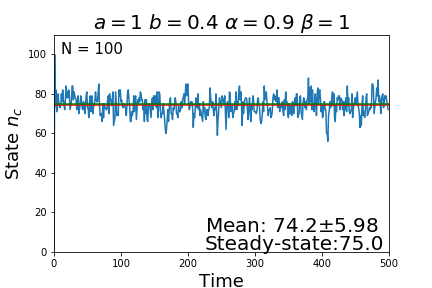
\includegraphics[width=\linewidth]{images/chapter3/ssA.png}
    \caption{A simulation with a steady state of 75. The average $n_{c}$ is close to the analytic value.}
  \end{subfigure}
  \begin{subfigure}[b]{0.4\linewidth}
    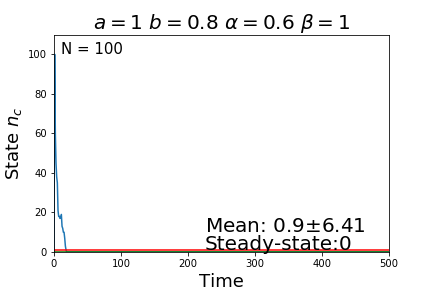
\includegraphics[width=\linewidth]{images/chapter3/ssB.png}
    \caption{A simulation with a steady state of 0. The average $n_{c}$ value is approximately $0$.}
  \end{subfigure}
  \caption{Sample simulations that compare the analytical steady-state of the given parameters and the mean $n_{c}$ value of the system.}
  \label{fig:compareSingleSS}
\end{figure}

$10$ sample runs were performed with different initial random number generator states and the final $n_{c}$ value for each iteration were recorded.
The mean and standard deviation of the simulated steady-state values are then computed for each parameter space $(\bar{a},b,\beta)$. 
The data points were then plotted with the corresponding parametrized differential curve shown in Fig.~\ref{fig:phase+sim}.
%All code used is provided in Appendix \ref{apndx:steadstatesim}, as well as 
More simulation experiments for various $b$ values are shown in Appendix \ref{apndx:ssexpt}

\begin{figure}[h!]
 \centering
  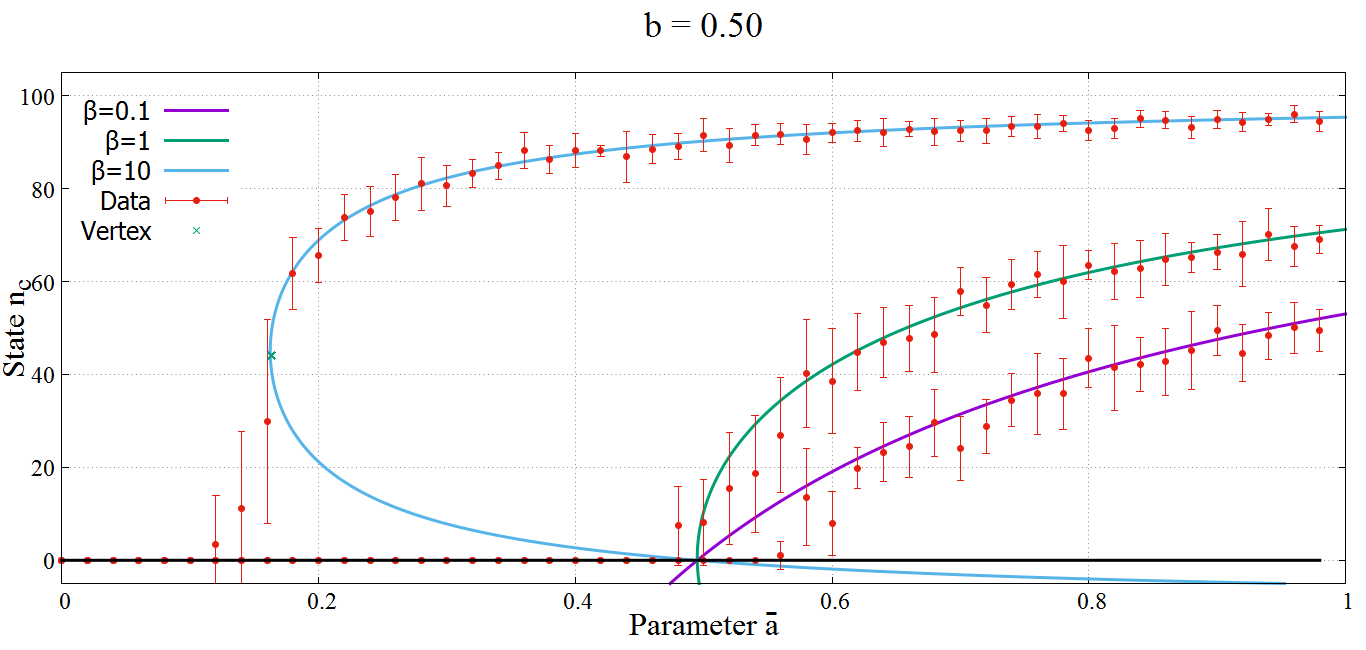
\includegraphics[width=\linewidth]{images/chapter3/phase+sim.png}
  \caption{The simulated steady-state values plotted against the analytic steady-state curves. The error bars provide the extent of deviation in simulations. The vertex is represented with the cross.}
  \label{fig:phase+sim}
\end{figure}

For $\beta \leq 1$, the simulation is consistent with the trivial steady state solution until it reaches the critical point $\bar{a} = b$, after which follows non-trivial, non-extraneous solution consistent with \eqref{eq:steadystate}.
Bifurcation occurs at $\bar{a}_1$.
For $\beta > 1$, the simulation follows the trivial steady-state and then breaks away and approaches the vertex of \eqref{eq:steadystate} at $\bar{a}_{2}$, after which, continues to follow the upper branch of \eqref{eq:steadystate}.
Bifurcation occurs somwhere before $\bar{a}_2$
The analytical solutions fail to predict the bifurcation from the trivial solution to the vertex of the curve.
Also, the significance of the lower branch for $\beta > 1$ curves is unknown and warrants further investigation.
The vertex is said to be unstable due to the fact that it unreliably and unpredictably settles to either trivial or non-trivial solution.
The lower branch may share this instability.    

\subsection{Unstable points}
\hspace{\parindent}For the previous simulation experiments, all agents start at state S and then forced to transition to state C. 
To investigate the properties of the lower branch on the non-trivial solution, we vary the number of agents that start the simulation in state C and remove the forcing function. 
This allows us to determine where the system will settle given the specific starting $n_{c}$ value, more particularly for $n_{c}$ values near the lower branch of the non-trivial solution. 
The code that generate the vector graphs is provided in Appendix %\ref{apndx:vectsim}

Shown in figure \ref{fig:vectorplot} are the new phase space graphs that include arrows that point to where that $n_{c}$ value for the given $\bar{a}$ settles.
More vector graphs are available in Appendix \ref{apndx:vectgraph}
The color of the arrows represents the probability of going towards that direction.
Intuitively for $\beta \leq 1$, all $n_{c}$ values point towards the trivial solution for all $\bar{a}$ values less than  $\bar{a}_{1}$ 100\% of the time. 
All $n_{c}$ with $\bar{a}$ values greater than $\bar{a}_{1}$ point towards the non-trival solution 100\% of the time.
For $\beta > 1$, what differs is the behavior at the vertex and the lower branch of the non-trivial solution.
$n_{c}$ values above the vertex have an estimated 50\% to either settle at the vertex or zero, while $n_{c}$ values below the vertex absolutely settle to zero.
Points slightly above the lower branch tend more towards settling to the upper branch but still have a chance to settle at 0.
Likewise for points below the lower branch.
Points within the lower branch have a 50\% of settling to either trivial or non trivial solution.
This means that coordinates near the lower non-trivial branch are unstable, since there is no certainty to which steady-state solution they will settle to.

\begin{figure}[h!]
 \centering
  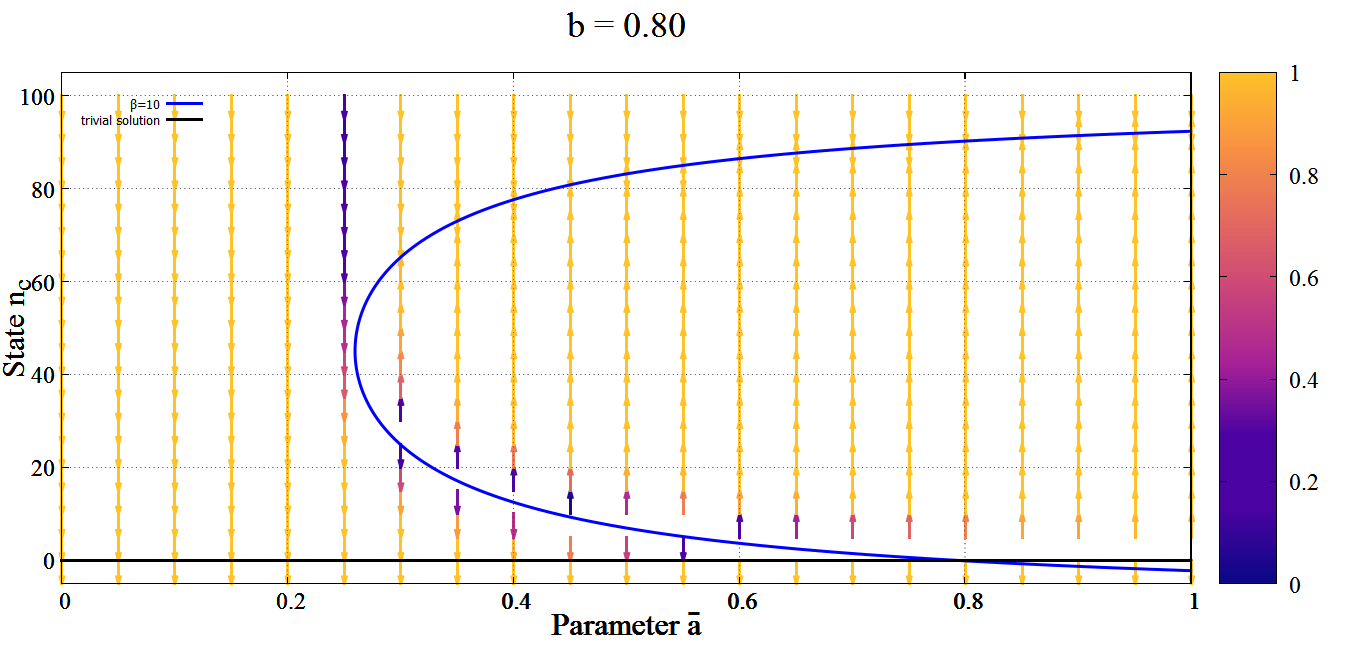
\includegraphics[width=\linewidth]{images/appendix/vectors/4.png}
  \caption{Vector graph for parameters $b = 0.8, \beta = 10$. The origin of the vector represents the initial $n_{c}$ and corresponding $\bar{a}$ value. The direction it points reveals whether it settles to the trivial or non-trivial solution. The color represents the probability of settling towards the directed steady-state.}
  \label{fig:vectorplot}
\end{figure}

%%

%\begin{figure}[htb]
%\centering
%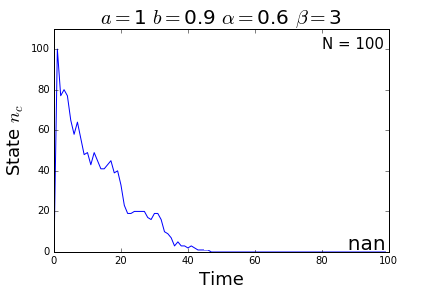
\includegraphics[width=0.3\columnwidth]{simulation/sim1}
%\includegraphics[width=0.3\columnwidth]{simulation/sim2}
%\includegraphics[width=0.6\columnwidth]{sim2}
%\caption{
%Sample simulations for $N = 100$ with the parameters: (a) $\bar{a} = 0.6$, $b = 0.9$ and $\beta = 3$ and (b) $\bar{a} = 0.36$, $b=0.7$ and $\beta = 14$.
%The simulation in (a) settles to the trivial steady-state ($n_{c}=0$) while the results in (b) show an average of $\langle{n_{c}}\rangle\approx85.5\pm 9.53$.
%[!! Remove the labels ``Steady State: ...''. One does not report an average with too many significant digits. What is the actual standard deviation (SD) here? Keep the decimal digits of the reported SD to two maximum.]
%(c) The average of the simulated steady-state values for different parameters are shown together with the theoretical predictions.
%The error bars provide the extent of the sample standard deviations computed. The cross indicates the vertex given by (9), i.e., $\bar{a_{2}}$
%} \label{fig:parametric}
%\end{figure}








